\documentclass[12pt]{report}
\usepackage{seminarka}
\usepackage{minted}
\usepackage{caption}

\addbibresource{references.bib}

\sloppy % oh well

\begin{document}



\pagenumbering{Roman}
\custtitlepage{Pokročilá kalkulačka}{[třída]}{ahi6}{Seminář z programování}{[škola]}{\today}

\renewcommand{\abstractname}{Anotace}
\begin{abstract}
Tato seminární práce se zabývá tvorbou pokročilé kalkulačky s grafickým uživatelským rozhraním. V rámci teoretické části práce jsem uvedl a popsal způsob převodu z infixové na postfixovou notaci a její následné vyhodnocení pro zaručení správného pořadí vykonaných výpočtů. Během praktické části jsem implementoval výslednou aplikaci v jazyce Rust za využití knihovny egui pro tvorbu grafického rozhraní. Touto prací jsem demonstroval využití teoretických matematických poznatků pro tvorbu užitečného počítačového programu.
\end{abstract}


% Ukázka stránky prohlášení

\declarationpage{
\pagenumbering{gobble}
    Prohlašuji, že tato seminární práce je mým původním autorským dílem, které jsem samostatně vypracoval. Všechny zdroje, odkazy a literatura použité nebo excerpované při zpracování této práce jsou řádně citovány a uvedeny v úplném odkazu na příslušný zdroj.
}{
    ahi6
    
    [místo], \today
}


\toc

\chapter{Úvod}

Kalkulačka je skvělým a užitečným nástrojem, jež umožňuje uživateli
provádět matematické výpočty velice snadno a rychle. Kromě základních
aritmetických operací mohou moderní kalkulačky disponovat mnoha
pokročilými funkcemi, které umožňují řešit složitější matematické úlohy.

Cílem mé seminární práce je navrhnout a následně implementovat
uživatelsky přívětivou kalkulačku, která kromě jednoduchých
aritmetických operací mezi dvěma čísly rovněž umí vyhodnotit celý
matematický výraz s ohledem na dodržení správného pořadí operací. Má
seminární práce tedy obsahuje popis algoritmů, které jsem se rozhodl pro
tento účel využít a konkrétní implementační detaily výsledné grafické
aplikace.

Toto téma jsem si vybral, protože implementace kalkulačky pro mě
představuje zajímavou výzvu, která mi umožní hlouběji porozumět, jakým
způsobem funguje tento základní program, a přitom využít teoretické
vědomosti z oblasti matematiky i praktické zkušenosti z oblasti vývoje
softwaru.

\chapter{Teoretická část}


%\section{Terminologie}
% není potřeba

\section{Analýza matematických
výrazů}

Nejběžnější způsob zápisu matematických výrazů, ve které se operátory
(``znaménka'') nachází mezi vstupními hodnotami (např. \(1+2\)), se
nazývá infixová notace \supercite{wiki:infixova_notace}. Ač je tento zápis pro člověka poměrně
intuitivní, pro stroj je mnohem obtížnější v tomto tvaru zapsaný
matematický výraz vyhodnotit, především z toho důvodu, že je v něm
komplikovanější určit správné pořadí, ve kterém je nutno dané operace
vykonat.

$$ 
1 + 2 \cdot 3 = 3 \cdot 3 = 9 \ \dots\ \text{špatné pořadí} 
$$

$$ 
1 + 2 \cdot 3 = 1 + 6 = 7 \ \dots\ \text{správné pořadí} 
$$


Proto je vhodné interně výraz převést do jiného zápisu, v mém případě
konkrétně do postfixové notace (též známé jako reverzní polská notace),
která na rozdíl od infixové notace umožňuje jednoznačně určit pořadí
operací bez nutnosti využití závorek ani složitých pravidel o precedenci
jednotlivých operací. Všechny vstupní hodnoty v tomto zápise předcházejí
operátor, díky čemuž lze správné pořadí odvodit již ze samotného
zápisu, protože víme, že hodnoty před daným operátorem nemohou být
využity jiným operátorem. Pro tento převod se využívá \textbf{Shunting
yard algoritmus}\supercite{brilliantShuntingYard} (v češtině známý též jako algoritmus \textit{seřaďovacího nádraží})\supercite{wiki:shunting_yard}, který byl poprvé popsán na začátku 60. let 20. století
slavným nizozemským informatikem Edsgerem Dijkstrou.\supercite{wiki:shunting_yard}

\begin{figure}
    \centering
    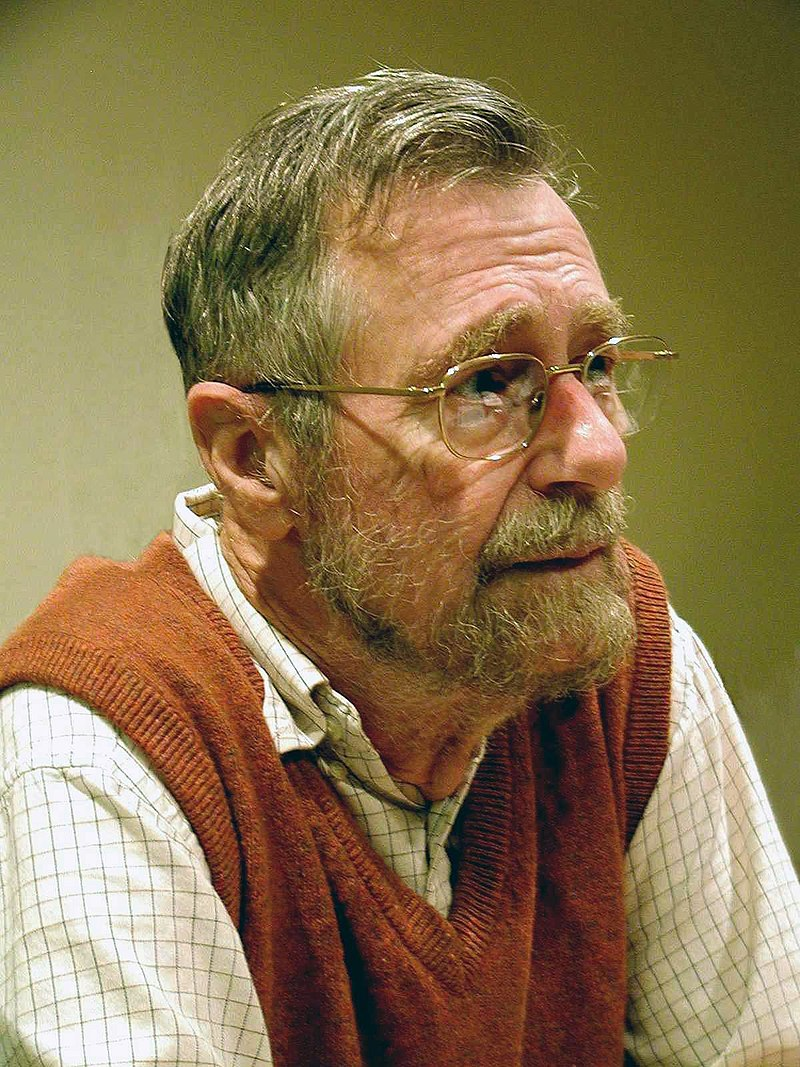
\includegraphics[width=0.4\linewidth]{800px-Edsger_Wybe_Dijkstra.jpg}
    \captionsetup{justification=centering}
    \caption[Edsger W. Dijkstra]{Edsger W. Dijkstra. \\
    Zdroj: Hamilton Richards, dostupné z \url{https://commons.wikimedia.org/w/index.php?title=File:Edsger_Wybe_Dijkstra.jpg&oldid=904110305} 
    %%\supercite{wiki:djikstra_foto} 
    } 
    \label{fig:enter-label}
\end{figure}

Princip tohoto algoritmu spočívá v tom, že vytvoříme zásobníky pro
jednotlivá čísla, operátory, a konečný výsledek, a potom výraz čteme
zleva doprava a postupujeme dle následujících pravidel: \supercite{geeksforgeeks_shutingYard}
\begin{enumerate}
	\item Pokud narazíme na číslici (nebo desetinnou tečku), zapíšeme si ji do
		zásobníku čísla

	\item Pokud narazíme na operátor, zásobník čísla převedeme na číslo typu float,
		vložíme jej do zásobníku pro konečný výsledek a zásobník čísla vyčistíme
		\begin{enumerate}
			\item Otevírací závorku vložíme do zásobníku operátorů

			\item Pokud narazíme na operátor, porovnáme jeho precedenci s operátorem
				na vrcholu zásobníku:
				\begin{itemize}
					\item Pokud má aktuální operátor vyšší precedenci než operátor na vrcholu
						zásobníku (nebo je zásobník prázdný), vložíme ho na zásobník

					\item Pokud má nižší nebo stejnou precedenci, vyjmeme operátory ze
						zásobníku a zapisujeme je na výstup, dokud nenarazíme na operátor s nižší
						precedencí nebo není zásobník prázdný
				\end{itemize}
		\end{enumerate}

	\item V případě znamének $+$ a $-$ navíc rozhodujeme, zda jsou operátory nebo
		součástí čísel podle toho, zda byl předchozí znak operátorem. (Pokud ano,
		tak znaménko považujeme za součást čísla)
\end{enumerate}

Pro zjednodušení moje implementace algoritmu předpokládá asociativitu
zleva doprava (což znamená, že operace jsou aplikovány zprava doleva),
která funguje pro většinu operací (až na umocňování, které potřebuje
rozlišovat také asociativitu zprava doleva.)\supercite{enwiki:1222245378}

Výsledný zásobník by měl obsahovat převedený zápis v postfixové notaci,
se kterým může kalkulačka dále pracovat. Je důležité zmínit, že moje
implementace algoritmu kontroluje pouze jednotlivé znaky vstupu, což
znamená že neumí spolehlivě rozpoznat chybně zadané rovnice a musí
spoléhat na to, že uživatel zadal rovnici správně, v opačném případě by
výsledný výstup byl nesmysl.

\section{Výpočet výrazu v postfixové
notaci}

Výpočet výrazu v postfixové notaci je poměrně snadný, lze vyřešit pomocí
jednoduchého algoritmu využívajícího zásobník. Stačí projít všechny
prvky výrazu zleva doprava\supercite{cvut:vyhodnoceni_vyrazu}; pokud je prvek číslem, je vložen do
zásobníku, a pokud je operátorem, tak se vyjmou poslední 2 hodnoty ze
zásobníku a výsledek dané operace na těchto hodnotách je do něj vložen
zpět. Na konci by měla v zásobníku zbýt pouze jedna hodnota, a to právě
výsledek výrazu. Pokud zbude v zásobníků více hodnot nebo pokud v
průběhu programu narazíme na nesrovnalost v počtu hodnot a operátorů,
považujeme vstup za nesprávný a uživateli vrátíme chybové hlášení.\supercite{wiki:postfix}

\chapter{Praktická část}

Pro tvorbu mojí aplikace jsem se rozhodl využít programovacího jazyka
Rust, jelikož umožňuje snadno vytvářet vysoce výkonné a přenositelné
aplikace.

Pro tvorbu grafického uživatelského rozhraní (anglicky GUI) jsem zvolil
knihovnu \emph{egui}, která se řadí k tzv. ``immediate mode'' GUI
knihovnám, které na rozdíl od obvyklých ``retained mode'' knihoven
neukládá komponenty uživatelského rozhraní do paměti, ale při každé
aktualizaci snímku je znovu vykreslit, což zvyšuje míru flexibility
rozhraní a zjednodušuje práci s interaktivními prvky na úkor výkonu
statických prvků rozhraní. V praxi to znamená, že lze vytvořit
sofistikované rozhraní za využití málo řádků kódu. Další žádoucí funkcí
knihovny egui je její rozsáhlá podpora různých druhů platforem, k nimž
patří Microsoft Windows, Mac OS, Linux, Android, iOS, popřípadě webový
prohlížeč prostřednictvím technologie WebAssembly.

\section{Struktura programu}

Stav mého programu je ukládán a organizován do struktury
\texttt{CalculatorApp}, která obsahuje tři důležité části: 
\begin{itemize}
    \item Text
vstupního pole \texttt{display\_text} pro zadávání výrazů a zobrazování
jejich výsledků 
    \item Případnou chybovou zprávu \texttt{error\_msg}, která
se uživateli zobrazí v případě že zadá chybný matematický výraz 
    \item Historie výpočtů \texttt{history}, která uchovává dynamické pole
obsahující veškeré výpočty provedené uživatelem společně s výsledky
Aplikace navíc implementuje ukládání stavu, což znamená, že si
kalkulačka pamatuje svůj předchozí stav i po uzavření programu, a to
včetně historie výpočtů. Toto je realizováno pomocí Rust knihovny
\texttt{serde}, která zajišťuje převod dat do formátu vhodného pro
uložení a opětovné načtení.
\end{itemize}

\begin{samepage}
\begin{minted}[frame=single,framesep=10pt,breaklines=true]{rust}
#[derive(serde::Deserialize, serde::Serialize)]
struct HistoryEntry {
    expression: String, // výraz
    result: String,     // výsledek
}

#[derive(serde::Deserialize, serde::Serialize)]
#[serde(default)]
pub struct CalculatorApp {
    display_text: String,
    error_msg: Option<String>, // chybová hláška je nastavena pouze tehdy, když nastane chyba
    history: Vec<HistoryEntry>, // dynamické pole záznamů historie
}
\end{minted}
\end{samepage}

Místo pevně daného rozložení tlačítek používá flexibilní systém, který
se přizpůsobuje velikosti okna. Metoda \texttt{calculator\_button\_row}
automaticky vypočítává šířku tlačítek podle dostupného prostoru, což
zajišťuje, že kalkulačka bude vypadat dobře na různých velikostech
obrazovky.

\begin{minted}[frame=single,framesep=10pt,breaklines=true]{rust}
fn calculator_button(&mut self, ui: &mut egui::Ui, label: &str, width: f32) {
    if ui
        // vykreslení tlačítka s dynamicky počítanou šířkou a pevně danou výškou
        .add(egui::Button::new(label).min_size( egui::vec2(width, 70.0)))
        .clicked() {
        // určité tlačítka mají speciální funkce
        match label {
            "C" => {
                // vymazat "displej" kalkulačky
                self.display_text.clear();
            }
            "=" => {
                // vypočítat výsledek a zobrazit jej
                let result = calculate(&self.display_text).map(|res| res.to_string());
                self.show_result(result);
            }
            "RPN" => {
                // převést výraz do reverzní polské notace
                let result = get_rpn(&self.display_text);
                self.show_result(result);
            }
            _ => {
                // ostatní tlačítka nemají žádné speciální funkce
                self.display_text += label;
            }
        }
    }
}
\end{minted}
\begin{minted}[frame=single,framesep=10pt,breaklines=true]{rust}
fn calculator_button_row(&mut self, ui: &mut egui::Ui, labels: &[&str]) {
    // šírku tlačítka vypočítáme jednoduchým podílem šířky obrazovky s počtem tlačítek
    let width = ui.available_width() / labels.len() as f32 - 8.0;
    ui.horizontal(|ui| {
        for label in labels {
            self.calculator_button(ui, label, width);
        }
    });
}
\end{minted}

\begin{minipage}{\textwidth}
Uživatelské rozhraní je tvořeno dvěma panely. Většinu prostoru zabírá ve výchozím stavu hlavní panel s tlačítky a vstupem/výstupem kalkulačky (a případně ještě chybovou hláškou), zbytek pak zabírá postranní panel s historií výpočtů, jehož šířka lze však dle potřeby nastavit uživatelem, což může být užitečné pro zobrazování obzvláště dlouhých matematických výrazů. Každý výpočet se zobrazuje ve sloupcích jako dvojice \texttt{výraz} = \texttt{výsledek}, a uživatel může kliknout na kterýkoli předchozí výraz nebo výsledek, aby ho znovu použil v jeho dalším výpočtu, což je velmi praktické při složitějších výpočtech, kde je nutné navázat na předchozí výsledek. Po dokončení výpočtů má uživatel možnost vymazat svoji historii, aby uvolnil místo pro nové budoucí výpočty a zjednodušil orientaci v historii.
\end{minipage}

\begin{figure}
    \centering
    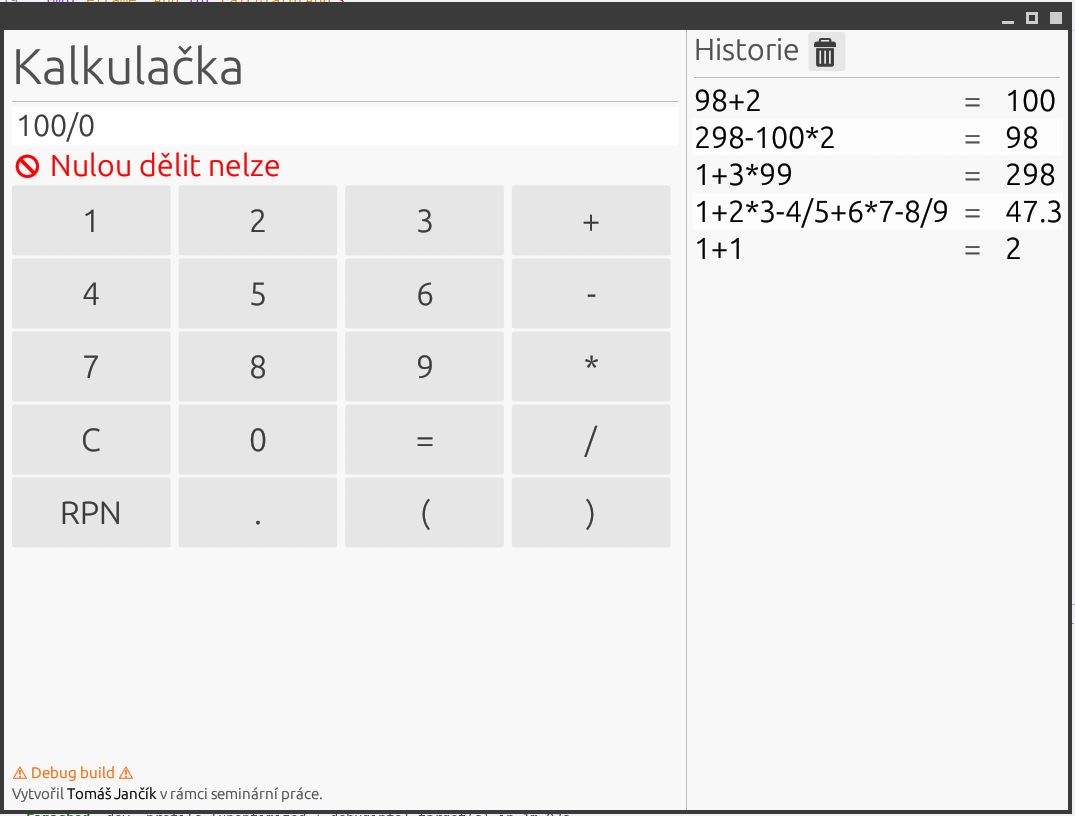
\includegraphics[width=1\linewidth]{Screenshot From 2025-01-02 12-01-35.png}
    \caption[Ukázka rozhraní běžícího programu]{Ukázka rozhraní běžícího programu. \\
    Zdroj: vlastní obrázek.}
    \label{fig:enter-label}
\end{figure}

\chapter{Závěr}

V rámci této seminární práce jsem úspěšně navrhl a implementoval pokročilou kalkulačku s grafickým uživatelským rozhraním. Program dokáže nejen provádět základní aritmetické operace, ale také vyhodnocovat komplexní matematické výrazy při dodržení správného pořadí operací.

Klíčovou součástí implementace byl Shunting yard algoritmus, jsem použil pro převod matematických výrazů z běžné infixové notace do postfixové notace. Tento převod významně zjednodušil proces vyhodnocování matematických výrazů a zajistil správné pořadí operací. Kromě samotných výpočtů program nabízí i možnost zobrazit výraz v postfixové notaci, což může být užitečné pro vzdělávací účely.

Vytvořená aplikace obsahuje řadu dodatečných praktických funkcí, které zvyšují její použitelnost. Mezi ty nejvýznamnější patří ukládání historie výpočtů, možnost znovu použít předchozí výrazy či výsledky, a flexibilní uživatelské rozhraní, které se přizpůsobuje velikosti okna. Díky využití programovacího jazyka Rust a knihovny egui je aplikace výkonná a přenositelná napříč různými operačními systémy.

Program splňuje všechny původní cíle, které jsem si stanovil na začátku práce. Přestože existuje prostor pro další vylepšení, například v podobě implementace pokročilejších matematických funkcí nebo robustnější kontroly vstupních výrazů, současná verze představuje plně funkční a praktický nástroj pro běžné matematické výpočty.

Práce na tomto projektu mi přinesla cenné zkušenosti v oblasti vývoje software a hlubší porozumění principům, na kterých fungují kalkulačky a vyhodnocování matematických výrazů. Zároveň jsem si vyzkoušel práci s moderními nástroji pro vývoj aplikací, jako je jazyk Rust a knihovna egui.

\printbibliography

\listoffigures

\end{document}
